\documentclass{article}
\title{\textbf{Introduction to Linux build systems}}
\author{}
\date{} 
\UseRawInputEncoding
\usepackage{graphicx}

% Links
\usepackage{hyperref}
\hypersetup{
    colorlinks=true,
    linkcolor=blue,
    filecolor=magenta,      
    urlcolor=cyan,
}
 
\urlstyle{same}

% Code Coloring
\usepackage{listings}
\usepackage{color}

\definecolor{dkgreen}{rgb}{0,0.6,0}
\definecolor{gray}{rgb}{0.5,0.5,0.5}
\definecolor{mauve}{rgb}{0.58,0,0.82}
\lstset{frame=tb,
  language=C++,
  aboveskip=3mm,
  belowskip=3mm,
  showstringspaces=false,
  columns=flexible,
  basicstyle={\small\ttfamily},
  numbers=none,
  numberstyle=\tiny\color{gray},
  keywordstyle=\color{blue},
  commentstyle=\color{dkgreen},
  stringstyle=\color{mauve},
  breaklines=true,
  breakatwhitespace=true,
  tabsize=3
}

\begin{document}
\maketitle
\tableofcontents{}
\section{The make utility and the make files}
It's an automatic build system, that drives the complier and generates an output executable files. and you need to know that in some situations in order to install a software in Linux, you just need to build it first from its source code.

\subsection{The build process}

\begin{center}
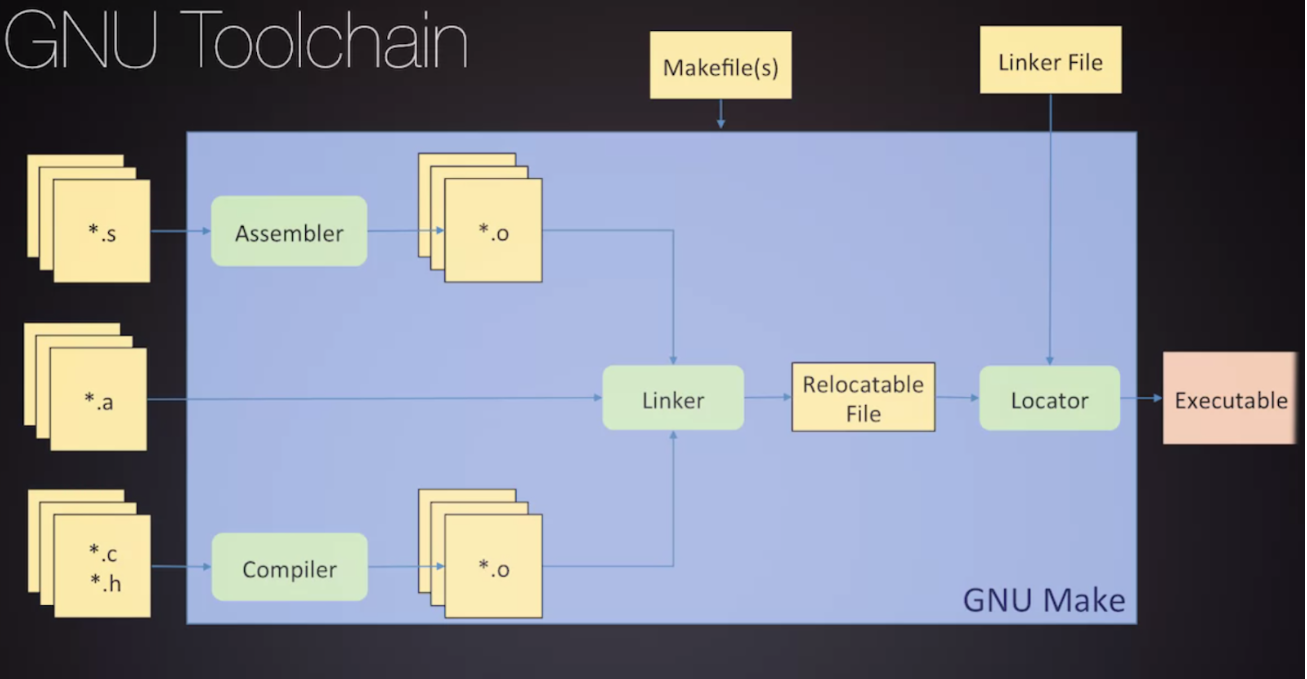
\includegraphics[scale=0.50]{./resources/imgs/build-process.png}
\end{center}

\subsection{makefile simple script}

\subsection{recipes, targets and dependencies}
The building process is a set of (rules), every rule might be dependent on another rule and so on.\\
A recipe can be constructed by a \textbf{target}, \textbf{dependencies or prerequisites}, and \textbf{command or recipe}

\begin{lstlisting}[language=make, caption=make rule structure]
[target ...] : [prerequisite ...]
    [recipe1]
    [recipe2]
\end{lstlisting}

Note: in \textit{make}, each line of a recipe starts with a TAB, and make sure it's a TAB as the \textit{make} util sometimes is sensitive to TABs and spaces while reading a recipe.\\

In order to invoke the \textbf{make.exe} to run, you can invoke with the following syntax:\\
\textit{make [option]... [target]... [macro=def]...}

\subsection{make implicit rules}

\subsection{make variables}
In make, we have two flavors of variables:
\begin{itemize}
    \item The value of a simply expanded variable is scanned once and for all, expanding any references to other variables and functions. It does not contain any references to other variables; it contains their values as of the time this variable was defined. (are expanded once at the time of the variable definition
    \item if it contains references to other variables, these references are expanded whenever this variable is substituted (in the course of expanding some other string). When this happens, it is called recursive expansion. (are expanded when the variable is substituted in)
Example:
\lstinputlisting[language=make, caption=building and linking with libraries]{./code/make/varaibles}

\end{itemize}

\subsubsection{make built-in variables}

\subsection{make built-in functions}

Note: You might need to visit the \href{https://www.gnu.org/software/make/manual/html_node/Functions.html}{\textit{make} documentation} for any all the list of the built-in functions.

\subsection{automatic variables}
These variables have values computed afresh for each rule that is executed, based on the target and prerequisites of the rule. It’s used to reduce the amount of typing in for a rule
\lstinputlisting[language=make, caption=building and linking with libraries]{./code/make/automatic-vars}

\subsection{Passing arguments to a makefile (Conditional Processing)}
Make allows you to use if conditions to change the build process and this means more flexibility

\lstinputlisting[language=make, caption=building and linking with libraries]{./code/make/make-conditional}

\subsection{Static pattern rules}
Static pattern rules are rules which specify multiple targets and construct the prerequisite names for each
target based on the target name.\\

{[target ]} : target-pattern : {[prerequisite-patterns ]}\\

The target specifies the targets the rules applies to. The target-pattern and prerequisite-patterns specify
how to compute the prerequisites of each target. Each target is matched against the target-pattern to
extract a part of the target name, called the stem. This stem is substituted into each of the
prerequisite-patterns to make the prerequisite names (one from each prerequisite-pattern).

\lstinputlisting[language=make, caption=building and linking with libraries]{./code/make/static-pattern-rules}


\subsection{special targets}

\subsection{Include other makefiles}
You can include other make files: usually a file for sources, and includes is made for the project, you can just use the \textit{include} directive

\section{Using Ninja build system}
Another types of build systems like \textbf{make} which is fast and lightweight and uses parallel builds.\\

Why Ninja: Ninja, a small build system with a focus on speed. It's built to be fast build system, and you will might notice that the speed will increase based on the CPU cores.

\subsection{Simple Ninja buid}
\lstinputlisting[caption=Simple build.ninja file]{./code/ninja/basic-example/build.ninja}

\lstinputlisting[caption=Ouput from Ninja build]{./code/ninja/basic-example/output}


\subsection{Generating Ninja files from code}
\subsubsection{Use misc/ninja\_syntax.py python script}

\subsubsection{Use meta-build system like cmake}

\section{intro to cmake} 
I think now you might asking what is really the difference between the cmake and the make environment.\\
The answer is the \textit{make} is a build system that drives the complier and the linker till the output executable is generated, but the \textit{cmake} is a cross-platform build system generator that can generate the makefiles themselves, then the role of the \textit{make} utility comes to build the software.\\

Simply \textbf{cmake} is meta-build system which is a build system that generates other build systems. (Note: Other meta-build systems like Gyn, and Gn).\\


\textit{cmake} is not only used for generating builds, but also it's used for packaging and installation!.

\subsection{minimal cmake program script}
\begin{lstlisting}[language=make, caption=Simple cmake script]
    cmake\_minimum\_required(VERSION 3.12)
    project(SimpleProject VERSION 1.0.0)
    
    add_executable(cmake-test main.cpp)
\end{lstlisting}

Generating and building the project:
\begin{lstlisting}[language=make, caption=Simple cmake script]
    cmake\_minimum\_required(VERSION 3.12)
    project(SimpleProject VERSION 1.0.0)
    
    add_executable(cmake-test main.cpp)
\end{lstlisting}

\begin{lstlisting}[language=make, caption=Building a simple cmake]
aramadan@CAI1-L11666  /c/Users/aramadan/Desktop/cmake
$ ls
build  CMakeLists.txt  main.cpp
    
aramadan@CAI1-L11666  /c/Users/aramadan/Desktop/cmake
$ cd build/

aramadan@CAI1-L11666  /c/Users/aramadan/Desktop/cmake/build
$ cmake -G 'MSYS Makefiles' ..
-- The C compiler identification is GNU 8.3.0
-- The CXX compiler identification is GNU 8.3.0
-- Check for working C compiler: C:/msys64/mingw64/bin/gcc.exe
-- Check for working C compiler: C:/msys64/mingw64/bin/gcc.exe -- works
-- Detecting C compiler ABI info
-- Detecting C compiler ABI info - done
-- Detecting C compile features
-- Detecting C compile features - done
-- Check for working CXX compiler: C:/msys64/mingw64/bin/g++.exe
-- Check for working CXX compiler: C:/msys64/mingw64/bin/g++.exe -- works
-- Detecting CXX compiler ABI info
-- Detecting CXX compiler ABI info - done
-- Detecting CXX compile features
-- Detecting CXX compile features - done
-- Configuring done
-- Generating done
-- Build files have been written to: C:/Users/aramadan/Desktop/cmake/build

aramadan@CAI1-L11666  /c/Users/aramadan/Desktop/cmake/build
$ cmake --build .
Scanning dependencies of target cmake-test
[ 50%] Building CXX object CMakeFiles/cmake-test.dir/main.cpp.obj
[100%] Linking CXX executable cmake-test.exe
[100%] Built target cmake-test

aramadan@CAI1-L11666  /c/Users/aramadan/Desktop/cmake/build
$ ./cmake-test.exe
Hello World!
\end{lstlisting}

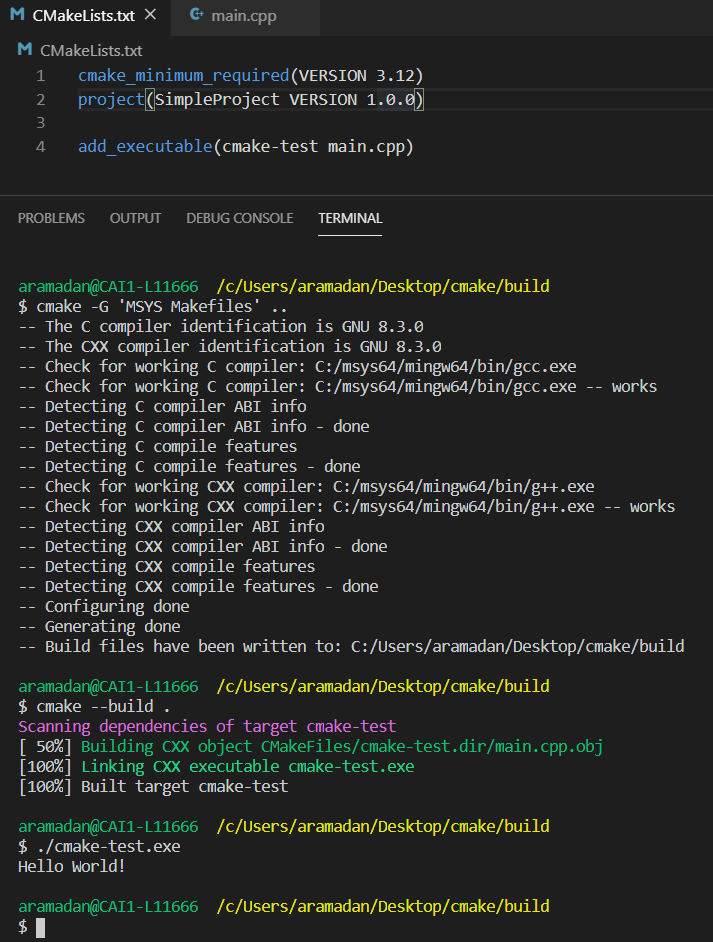
\includegraphics[scale=0.75]{./resources/imgs/cmake/build-simple-cmake.PNG}

You can also build and link with libraries, let's consider that we have a new files \textbf{"libfoo.hpp, and libfoo.cpp"} and let's print the hello world from inside.
\lstinputlisting[language=bash, caption=building and linking with libraries]{./code/cmake/build-and-link-libs/build-and-link-libs}

the output as expected, but let's see how can we edit the CMakeLists file.
\lstinputlisting[language=bash, caption=building and linking with libraries]{./code/cmake/link-cmakelists}

\subsection{Adding sub-directories (Including other CMakeLists.txt)}
You can add sub-directory to be combined with the current while building. you can achieve that by adding creating a new sub-directory and creating a separate CMakeLists for it, then using the \textbf{add\_subdirectory(directory\_name)} inside the main CMakeLists.txt.


Interface Modes
\begin{itemize}
    \item Public
    In \textbf{PUBLIC} interface, Any one links with the library will be have the includes also the all the directives visible to him. 
    \item Private 
    In \textbf{PRIVATE} only us has the ability to see our definitions
    \item Interface 
    In \textbf{INTERFACE} We can't see the definitions, only our consumers.
\end{itemize}

\subsection{cmake generators}
\textit{cmake} is a cross-platform generator which allows generating a complete build environment, and you can not only using it for generating a makefiles but you can use also to generate other build environments templates for XCode, Visual Studio, Ninga build, ... etc.
and you can achieve using a certain generate by specifying it using \textbf{'-G'} option.

\begin{lstlisting}[language=make, caption=Using a specific generator]
aramadan@CAI1-L11666  /c/Users/aramadan/Desktop/cmake/build
$ cmake -G 'MSYS Makefiles' ..
# Here we are using a makefiles under the MSYS environment
\end{lstlisting}

Note: for a list of all the generators use \textit{\textbf{cmake -G}} 

\subsubsection{Using the cmake to generate for Visual Studio}
As we just discussed you can use \textit{cmake} to generate Visual Studio projects by specifying a certain generator. the next example will show that.
\lstinputlisting[language=make, caption=building and linking with libraries]{./code/cmake/vs2015-log}

The output is a normal visual studio 2015 solution as follow:

\begin{center}
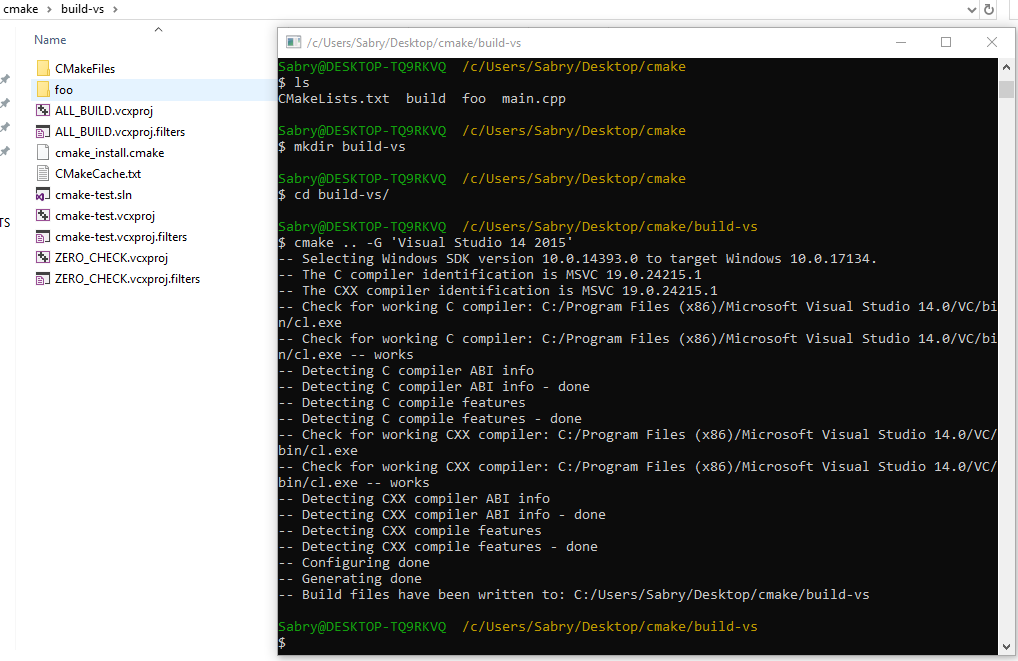
\includegraphics[scale=0.50]{./resources/imgs/cmake/vs2015-generator.PNG}
\end{center}

You can normally open the solution with the visual studio, and you might notice that the \textit{cmake} has generated four projects as follow;
\begin{center}
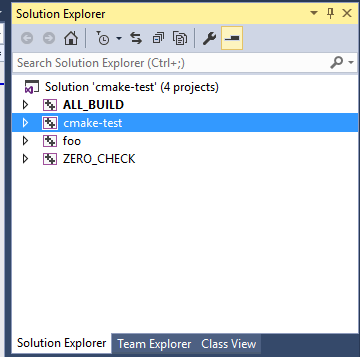
\includegraphics[scale=0.65]{./resources/imgs/cmake/openin-vs2015.PNG}
\end{center}
two of them are our foo library and the other is the cmake-test project, but what about the \textbf{ALL\_BUILD}, and \textbf{ZERO\_CHECK} projects.

\begin{itemize}
    \item ALL\_BUILD project is used to build every signal project in the solution, you can think of it as \textit{make all}
    \item ZERO\_CHECK is used to sync with the original CMakeLists.txt file, so if you changed anything in the CMakeLists.txt you should build this project to sync with the visual studio solution.
\end{itemize}

\textit{cmake} can be used to generate a lot of build systems, such that \textit{make} build files, or XCode projects, even visual studio projects ... etc.

\end{document}